%% LyX 2.1.1 created this file.  For more info, see http://www.lyx.org/.
%% Do not edit unless you really know what you are doing.
\documentclass[english]{llncs}
\usepackage[T1]{fontenc}
\usepackage[latin9]{inputenc}
\usepackage{color}
\usepackage{array}
\usepackage{verbatim}
\usepackage{url}
\usepackage{multirow}
\usepackage{graphicx}

\makeatletter

%%%%%%%%%%%%%%%%%%%%%%%%%%%%%% LyX specific LaTeX commands.
%% Because html converters don't know tabularnewline
\providecommand{\tabularnewline}{\\}

%%%%%%%%%%%%%%%%%%%%%%%%%%%%%% User specified LaTeX commands.
\usepackage{algorithmic}

\@ifundefined{showcaptionsetup}{}{%
 \PassOptionsToPackage{caption=false}{subfig}}
\usepackage{subfig}
\makeatother

\usepackage{babel}
\begin{document}
\title{Evaluation of Query Reformulation Methods for Patent Prior Art Search with Partial Patent Applications}
\maketitle
\begin{abstract}
Patents are used by entities to legally protect their inventions and
represent a multi-billion dollar industry of licensing and litigation.
In 2012, 276,788 patent applications were approved in the US alone
-- a number that has doubled in the past 15 years. While much of the
literature inspired by the evaluation framework of the CLEF-IP competition
has aimed to assist patent examiners in assessing prior art for complete
patent applications, less of this work has focused on patent search
with queries representing (partial) applications to help inventors
to assess the patentability of their ideas prior to writing a full
application. %Hence, in this paper, we focus on both helping inventors to assess the patentability of their ideas and patents examiners to assess the patentability of a given patent application.
In this paper, we carry out an intensive study and evaluation of both
patent specific and standard query reformulation methods for patent
prior art search with partial patent applications.
\end{abstract}

\begin{keywords} Query Reformulation, Patent Search, Experimentation.
\end{keywords} 


\section{Introduction}

\noindent Patents are used by entities to legally protect their inventions
and represent a multi-billion dollar industry of licensing and litigation.
In 2012, 276,788 patent applications were approved in the US alone
a number that has doubled in the past 15 years. Hence, helping both
inventors and patent examiners assess the patentability of a given
patent application through a patent prior art search is a critical
task.

Patent prior art search involves finding previously granted patents
that may be relevant to a new patent application. The objective and
challenges of standard formulations of patent prior art search are
different from those of standard text and web search since~\cite{Magdy2012}:
(i) queries are (partial) patent applications, which consist of documents
with hundreds of words organized into several sections, while queries
in text and web search constitute only a few words; (ii) patent prior
art search is a recall-oriented task, where the primary focus is to
retrieve all relevant documents at early ranks, in contrast to text
and web search that are precision-oriented, where the primary goal
is to retrieve a subset of relevant documents. Another important characteristic
about patent patent prior art search is that, in contrast to scientific
and technical writers, patent writers tend to generalize and maximize
the scope of what is protected by a patent, %by using a combination of abstract and specific terminology, 
and try to make sure that finding any relevant prior work by the patent
examiner is a hard job.

While much of the literature inspired by the evaluation framework
of the CLEF-IP competition has aimed to assist patent examiners in
assessing prior art for complete patent applications, less work has
focused on assessing the patentability of inventions before writing
a full patent application. Prior art search with queries that represent
unfinished patent applications is certainly desirable, since writing
a full application is time-consuming and costly, especially if lawyers
are hired to assist.

%However prior art search with partial applications is much different than queries with a full application -- namely because the queries are much shorter and represent only parts of a patent application.

%NOTE: start a paragaph with the key idea%A patent application is organized in, at least, four sections: title,%abstract, claims and description. We assumed that a partial application%consist in one of the mentioned sections. 

To assess the difficulty of querying with partial patent applications,
we refer to Figure~\ref{fig:FailureAnalysis}. Here we show an analysis
of the average Jaccard similarity%
\footnote{The Jaccard similarity is used to measure the term overlap between
two sets, and is defined as the size of the intersection divided by
the size of the union of the sample sets. Before applying the Jaccard
similarity, patent-specific stopwords were removed, as suggested by
\cite{Mahdabi2012}.%
} between different queries (representing the title, abstract, claims,
or descriptions intended to represent a partial patent application)
and the labeled relevant (all) and irrelevant documents (top 10 irrelevant
documents ranked by BM25~\cite{Robertson1993}). We show results
for the top 100 and bottom 100 queries (100 queries that perform the
best, and 100 queries that perform the worst) of CLEP-IP 2010 evaluated
according to Mean Average Precision (MAP). Note that, while the title
section is usually composed by an average of six terms, the other
sections are longer, ranging from ten to thousands of terms.

\begin{figure}[!th]
\begin{centering}
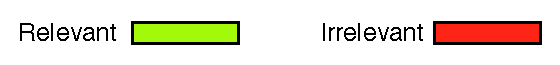
\includegraphics[width=6cm]{img/legend} 
\par\end{centering}

\begin{centering}
\subfloat[Title query.]{\begin{centering}
\includegraphics[width=2.9cm]{Results-CIKM2014/jaccard-qTitle-CLEF-IP2010} 
\par\end{centering}

}\subfloat[Abstract query.]{\begin{centering}
\includegraphics[width=2.9cm]{Results-CIKM2014/jaccard-qAbstract-CLEF-IP2010} 
\par\end{centering}

}\subfloat[Claims query.]{\begin{centering}
\includegraphics[width=2.9cm]{Results-CIKM2014/jaccard-qClaims-CLEF-IP2010} 
\par\end{centering}

}\subfloat[Description query.]{\begin{centering}
\includegraphics[width=2.9cm]{Results-CIKM2014/jaccard-qDescription-CLEF-IP2010} 
\par\end{centering}

}
\par\end{centering}

\centering{}\protect\caption{Average Jaccard similarity of (ir)relevant documents with the result
sets for different queries. }
{\footnotesize{}\label{fig:FailureAnalysis}}
\end{figure}


There are three notable trends here: (i) term overlap increases from
title to description since the query size grows accordingly; (ii)
the bottom 100 performing queries tend to have much smaller term overlap
with the relevant documents than the top 100 queries; and (iii) the
best overlap for any relevant document set for any set of queries
is less than one in four terms. Therefore, we suggest an investigation
of \emph{query reformulation} \cite{Baeza-Yates2010} methods as a
means for improving the term overlap between queries that represent
partial patent applications and relevant documents, with the objective
of assessing not only the performance of standard query reformulation
methods, but also the effectiveness of query reformulation methods
that exploit patent-specific characteristics. In this paper, we try
to mainly answer the following questions: \emph{What are these patent
query reformulation methods and how do they work? What is the best
section in a patent application to use as a query? What is the best
patent query reformulation method? To which extent are they efficient
compared to standard query reformulation approaches?}

The main contributions of this work can be summarized as follows:
\begin{enumerate}
\item We propose a deep study of the state of the art patent query reformulation
methods.
\item A thorough comparative analysis of these methods against standard
query reformulation methods on standardized datasets of CLEF-IP. 
\end{enumerate}
The rest of the paper is organized as follows: in Section \ref{sec:QueryReformulation}
we present a set of patent specific query reformulation methods; in
Section \ref{sec:evaluation} we present our evaluation framework
and results analysis; and in Section \ref{sec:conclusion} we conclude
with possible directions for future work.

%Query Reformulation is the process of transforming an initial query $Q$ to another query $Q'$. This transformation may be either a reduction or an expansion of the query. \emph{Query Reduction} (QR) \cite{Kumaran2009} reduces the query such that superfluous information is removed, while \emph{Query Expansion} (QE) \cite{Efthimiadis1996} enhance the query with additional terms likely to occur in relevant documents. 

%Therefore, we investigate the impact of query reduction methods when querying with long sections such as abstract, claims or description. 

%As already mentioned, Query Expansion (QE)~\cite{Efthimiadis1996} is a query reformulation approach that adds terms to an initial query in order to improve retrieval performance. The utility of QE for patent prior art search is motivated by the term overlap analysis depicted in Figure \ref{fig:FailureAnalysis}, which illustrates that there is a large term mismatch between queries an relevant documents. This term mismatch may be alleviated by QE methods.

% The following is a reasonable argument, but could be refuted by% reviewers... term coverage and recall are more direct and simple% arguments.

%In summary, the contributions of this paper are the following:  %\begin{enumerate}%\item Novel contributions for query expansion and reduction that leverage%(a) patent structure and (b) term diversification techniques. %\item A thorough comparative analysis of existing and novel methods for%query expansion and reduction in patent prior-art search on standardized%datasets of CLEF-IP. %\end{enumerate}



\begin{comment}

\section{Related work}

\label{sec:relatedworks}

\textcolor{red}{Gaby said: this section should be shorter (}\textcolor{blue}{Reda:
Why?}\textcolor{red}{)}

Query Reformulation is the process of transforming an initial query
$Q$ to another query $Q'$. This transformation may be either a reduction
or an expansion of the query. \emph{Query Reduction} (QR) \cite{Kumaran2009}
reduces the query such that superfluous information is removed, while
\emph{Query Expansion} (QE) \cite{Efthimiadis1996} enhance the query
with additional terms likely to occur in relevant documents.

%The major contributions in patent search has focused on query formulation, where the objective is to find the best terms to represent a patent application as a query to achieve high retrieval effectiveness by retrieving all possible relevant documents at high ranks \cite{Magdy2012}. 

%The scenario of patent prior art search consists of manually form queries by selecting high frequency terms from patent application. Hence, following this methodology, some algorithms of patent query reduction have been proposed to select only useful terms from patent application \cite{Ganguly2011,Itoh2003}. We used the approach propose by Ganguly et al. \cite{Ganguly2011} for QR as a baseline, and we showed that the performance of MMRQR outperform this approach in many cases. 

------

There are a variety of existing query expansion methods that use synonyms
(both from WordNet and automatically generated)~\cite{Magdy2011},
by supervised learning~\cite{Bashir2010}, by IPC codes (a variant
on our baseline approach that additionally uses the citation network
of patents)~\cite{Verma2011}, and a query-specific patent lexicon
based on the definitions of the IPC~\cite{Mahdabi2013}. While our
intention in this paper was to comprehensively evaluate very general
methods for QE using \emph{partial patent applications}; it would
be interesting future work to comprehensively evaluate all of these
patent-specific QE methods with our generic methods for partial patent
application queries. 

--------

Classical query expansion methods has been used for prior art search
by Magdy et al. \cite{Magdy2011}, which rely on pseudo-relevance
feedback and WordNet as source of expansion terms. However, none of
these approaches were able to achieve a significant improvement over
the baseline. Therefore, they introduce a novel approach that automatically
generates synonym sets for terms, and use them as a source of expansion
terms, which showed significant improvement with respect to the baseline.
Also, Bashir et al. \cite{Bashir2010} propose a query expansion with
pseudo-relevance feedback. Query expansion terms are selected using
a using a machine learning approach, by picking terms that may have
a potential positive impact on the retrieval effectiveness. However,
this approach can be computational expensive, since the presented
features are complicated to compute, e.g. Pair-wise Terms Proximity
features. Verma and Varma \cite{Verma2011} propose a different approach,
which instead of using the patent text to query, use its International
Patent Classification (IPC) codes, which are expanded using the citation
network. The formed query is used to perform an initial search. The
results are then re-ranked using queries constructed from patent text.
Throughout our experiments, we concluded that relying on non-patent
terms to expand a query, leads to poor retrieval quality. 

Also query reduction methods have been applied in order to deal with
long queries, which are composed by full patent applications \cite{Ganguly2011,Itoh2003}.
Even these methods are interesting, they are not suited to deal with
short queries (partial patent applications). Recently, \cite{Mahdabi2013}
proposed as reduction process to short the query by taking only the
first claim of a patent application since it contains the core of
the invention. This approach has not been implemented as its authors
already point out its poor performance.
\end{comment}



\section{Query Reformulation for Patents}

\label{sec:QueryReformulation}

%In this section, we first present the requirements of a query expansion method in Sections \ref{sec:FrameworkQE}, then, we introduce a novel term selection method for query expansion in Section \ref{sec:MMRQE}. Next, in Section \ref{sec:FrameworkQR} we introduce the motivations behind the benefit of query reduction, and a new approach of query reduction in Section \ref{sec:MMRQR}.

Query Reformulation is the process of transforming an initial query
$Q$ to another query $Q'$. This transformation may be either a reduction
or an expansion of the query. \emph{Query Reduction} (QR) \cite{Kumaran2009}
reduces the query such that superfluous information is removed, while
\emph{Query Expansion} (QE) \cite{Efthimiadis1996} enhance the query
with additional terms likely to occur in relevant documents. 

\begin{comment}
During the exploration of query reformulation for patent search with
partial patent applications, there are many configuration options
and associated questions that we considered:
\begin{description}
\item [{Query type:}] We consider that a query of a partial patent application
consist of either the title, the abstract, the claims or the description
section. A critical question is what part of a partial application
an inventor should write to obtain the best search results? 
\item [{Relevance model:}] We explore a probabilistic approach represented
by the popular BM25~\cite{Robertson1993} algorithm, as well as a
vector space model (VSM) approach, TF-IDF~\cite{Salton1975}. A natural
question is which relevance model works best for query reformulation
for patent prior art search?
\item [{Query expansion source:}] In the case of query expansion, we consider
the abstract, claims, and description sections as different term sources
to determine which section offers the best source of expansion terms,
e.g., are the claims words of particularly high value as expansion
terms? 
\item [{Term selection method:}] We consider different term selection
methods for query reformulation. Then a natural question is, which
term selection method works best, and with which configuration, i.e.
query type, retrieval model, and term source for query expansion methods? \end{description}
\end{comment}



\subsection{Patent Query Expansion Methods}

In this paper, we consider four patent specific query expansion methods,
that we believe are the most representative.


\subsubsection{Maximal Marginal Relevance for Patent Query Expansion}

\begin{comment}
As a term selection method in QE, Rocchio derives a score for each
potential query expansion term and in practice, the top-$k$ scoring
terms (often for $k\ll200$) are used to expand the query and are
weighted according to their Rocchio score during the second stage
of retrieval. The caveat of this approach is that given a limited
budget of $k$ expansion terms, there is no inherent guarantee that
these terms ``cover'' all documents in the pseudo-relevant set.
\end{comment}
{} 

In this case, we want to define a method of ``diverse'' term selection
--- such as the \emph{Maximal Marginal Relevance} (MMR)~\cite{Carbonell1998}
algorithm for result set diversification. The idea is to use it for
diverse term selection. In the case of query expansion, we call this
method MMRQE.

%\subsubsection{MMR Query Expansion (MMRQE)}
%\label{sec:MMRQE}


%%%%%%%%%%%%%%%%%%%%%%%%%%%%%%%%%%%%%%%%%%%%%%%%%%%%%%%%%%%%%%%%%%%%%
\begin{figure}[!h]
\begin{centering}
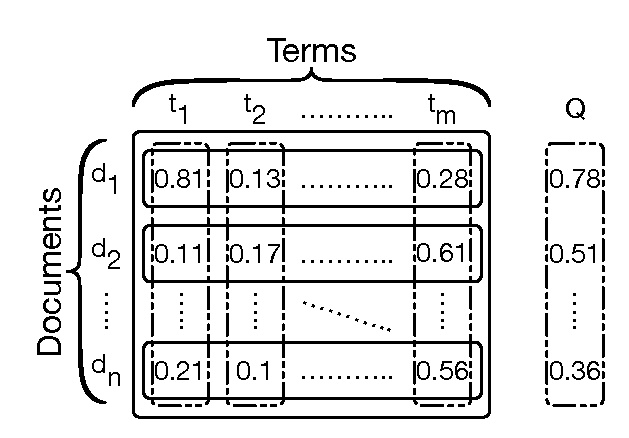
\includegraphics[width=5cm]{img/matrix} 
\par\end{centering}

\protect\caption{Notation used in MMR QE/QR.}


\label{fig:notation} 
\end{figure}


%%%%%%%%%%%%%%%%%%%%%%%%%%%%%%%%%%%%%%%%%%%%%%%%%%%%%%%%%%%%%%%%%%%%%


MMRQE takes as input a pseudo-relevant feedback set of $n$ documents
(PRF), which is obtained after a retrieval for the initial query.
From the PRF set, we build a document-term matrix of $n$ documents
and $m$ terms as shown in Figure~\ref{fig:notation}, which uses
a TF-IDF weighting for each document vector (row $d_{i}$ for $1\leq i\leq n$).
However, as we will see shortly, the view that will be important for
us in this work is instead the term vector (column $t_{j}$ for $1\leq j\leq m$).
To represent the query $Q$ column vector in Figure~\ref{fig:notation}
having a numerical entry for every document $d_{i}$, we found that
computing the BM25 or TF-IDF score between each document $d_{i}$
and the query provided the best performance (in our experiments, the
score used is given by the indicated relevance model).

Given a query representation $Q$, we aim to select an optimal subset
of $k$ terms $T_{k}^{*}\subset D$ (where $|T_{k}^{*}|=k$ and $k\ll|m|$)
relevant to $Q$ but inherently different from each other (i.e., diverse).
This can be achieved by building $T_{k}^{*}$ in a greedy manner by
choosing the next optimal term $t_{k}^{*}$ given the previous set
of optimal term selections $T_{k-1}^{*}=\{t_{1}^{*},\ldots,t_{k-1}^{*}\}$
(assuming $T_{0}^{*}=\emptyset$) using the MMR diverse selection
criterion.


\subsubsection{Synonyms Sets for Patent Query Expansion}

Magdy et al. \cite{Magdy2011} proposed a patent query expansion method,
which automatically generates candidate synonyms sets (SynSet) for
terms, and use it as a source of expansion terms. The idea for generating
the SynSet comes from the characteristics of the CLEF-IP patent collection,
where some of the sections in some patents are translated into three
languages (English, French, and German). The idea is to use these
parallel manual translations to create possible synonyms sets. Hence,
for a word $w$ in one language which has possible translations to
a set of words in another language ${w_{1},w_{2},\ldots,w_{n}}$,
this set of words can be considered as synonyms or at least related
to each other. The generated SynSet is used for query expansion in
two ways: (i) The first one use the probability associated with the
SynSet entries as a weight for each expanded term in the query (denoted
\textbf{WSynSet}). Therefore, each term was replaced with its SynSet
entries with the probability of each item in the SynSet acting as
a weight to the term within the query. (ii) The second one neglected
this associated probability and used uniform weighting for all synonyms
of a given term (denoted \textbf{USynSet}). This strategy is similar
to adding synonyms from WordNet where no probability is assigned.


\subsubsection{Patent Lexicon for Query Reformulation}

Mahdabi et al. \cite{Mahdabi2013} proposed to build a query-specific
patent lexicon based on definitions of the International Patent Classification
(IPC). The lexicon is simply build by removing general and patent
stop-words from the text of IPC definition pages. Each entry in our
lexicon is composed of a key and a value. The key is an IPC class
and the value is a set of terms representing the mentioned class.
Then, the lexicon build is used to extract expansion concepts related
to the context of the information need of a given query patent. To
this end, the IPC class of the query patent is searched in the lexicon
and the terms matching this class are considered as candidate expansion
terms. %
\begin{comment}
Query expansion using the lexicon is expected to solve the two problems:
(i) The first problem is related to the fact that the usage of words
is sensitive to the topic domain; In different domains, the same word
may be used to indicate different meanings. We aim at finding the
correct sense of a word, by associating relevant terms from the topic
domain to the given query terms for each query patent. (ii) The second
problem is related to the term mismatch. The vocabulary of the query
patent is tailored by the language usage of the author (a non-standard
terminology), while conceptual lexicon provides a more standard terminology.
\end{comment}
{} The approach proposed tries to combine these two complementary vocabularies.
In this paper we refer to this patent query expansion method as \textbf{IPC
Codes}.


\subsection{Patent Query Reduction Methods}

Here, consider the following three patent query reduction methods.


\subsubsection{Maximal Marginal Relevance for Patent Query Reduction}

Following the same motivations than those of explore diversification
for term selection, we can imagine greedily rebuild the query from
scratch, while choosing diversified terms (i.e. terms of the query).
Here, we call this approach MMR Query Reduction (MMRQR). Formally,
given a query representation $Q$, we aim to select an optimal subset
of $k$ terms $T_{k}^{*}\subset Q$ (where $|T_{k}^{*}|=k$ and $k<|Q|$)
relevant to $Q$ but inherently different from each other (i.e., diverse).
This can be achieved by building $T_{k}^{*}$ in a greedy manner by
choosing the next optimal term $t_{k}^{*}$ given the previous set
of optimal term selections $T_{k-1}^{*}=\{t_{1}^{*},\ldots,t_{k-1}^{*}\}$
(assuming $T_{0}^{*}=\emptyset$) using an adaptation of the MMR diverse
selection criterion. Note that the we used all the sections of the
patent documents of the PRF set to built the document-term matrix
of $n$ documents and $m$ terms shown in Figure~\ref{fig:notation}.


\subsubsection{Language Model for Query Reduction}

In \cite{Ganguly2011}, the authors proposed a query reduction technique,
which decomposes a query (a patent section) into constituent text
segments and computes a Language Modeling (LM) similarities by calculating
the probability of generating each segment from the top ranked documents
(PRF set). Then, the query is reduced by removing the least similar
segments from the query. We refer to this method by \textbf{LMQR}.


\subsubsection{IPC Codes for Query Reduction}

Based on the intuition that, terms in the IPC code definition may
represent \textquotedbl{}stop-words\textquotedbl{}, especially if
they are rare (infrequent in the patent application), one can think
to reduce a patent query as follows: (i) For each patent application,
take the definitions of the IPC codes which are associated to it.
Then, (ii) rank the terms of the query according to both their frequency
in the class code definition, and their frequency in the query. Finally,
(iii) remove bottom terms of this ranking from the query (i.e. good
terms are terms that occur a lot in the query, and few in the class
code definition, whereas bad terms are those that occur few in the
query, and a lot in the class code definition). In the evaluation
section we denote this approach \textbf{IPC Codes}. 

\begin{comment}
In the next section, we propose a deep evaluation of the above query
reformulation methods.
\end{comment}


%for patent search, and we attempt to answer the questions we asked in the beginning of this section.


\section{Experimental Evaluation}

\label{sec:evaluation} 

In this section, we discuss the results of the evaluation performed
on the query reformulation methods described above.


\subsection{Experimental Setup}

\label{sec:setup}

For our experiments we used used the Lucene IR System%
\footnote{\texttt{http://lucene.apache.org/}%
} to index the English subset of CLEF-IP 2010 dataset%
\footnote{\texttt{\url{http://www.ifs.tuwien.ac.at/~clef-ip/}}%
}~\cite{Piroi2011,Roda2009} with the default stemming and stop-word
removal. We removed patent specific stop-words as described in \cite{Magdy2012}.
CLEF-IP 2010 contains 2.6 million patent documents, and the English
test sets of CLEF-IP 2010 correspond to 1303 topics. We also made
the same experiments on the CLEF-IP 2011 dataset, but for lack of
space we omit the results from the paper. However the obtained results
was almost similar and presented the same trends.

In our implementation, each section of a patent (title, abstract,
claims, and description) is indexed in a separate field. Hence, when
a query is processed, all fields in the index are targeted, since
it is sensible to use all available content. We also used the patent
classification (IPC) for filtering the results by constraining them
to have common classifications with the patent topic as suggested
in previous works \cite{Lopez2009,Roda2009}. Finally, we report MAP,
and PRES \cite{Magdy2010a}, which combines Recall with the quality
of ranking and weights relevant documents lower in the ranking more
highly than MAP. We report the evaluation metrics on the top 1000
results.

\textcolor{red}{}%
\begin{comment}
\textcolor{red}{Gabi said: a review from ckim commented that the ipc
filter could be too restricted taking into account that patent applications
usually dont contained revised ipc codes. But, if I remembered correctly,
when you turn off the filter the results were no significant different
and you decided to keep the filter on, since the systems works faster.
Is that true? . If yes, we should commented in the paper.}
\end{comment}


\begin{comment}
\begin{figure}[!h]
\begin{centering}
\includegraphics[width=4cm]{analysis/precision-recall_ByField-CLEF-IP_2010.eps}\includegraphics[width=4cm]{analysis/MAP-MRR_ByField-CLEF-IP_2010.eps}
\protect\caption{The utility of query reduction for 1304 abstract queries of the CLEF-IP
2010 dataset. }

\par\end{centering}

\begin{centering}
{\footnotesize{}{}\label{fig:QRUtility}} 
\par\end{centering}

{\footnotesize{}{}%different queries (representing the title, abstract, or claims of a patent application)%and the labeled (ir)relevant documents for the best (top) and worst (bottom) performing%queries from CLEF-IP 2010 w.r.t. MAP.}} 
\end{figure}
\end{comment}


%\begin{figure}%\begin{centering}%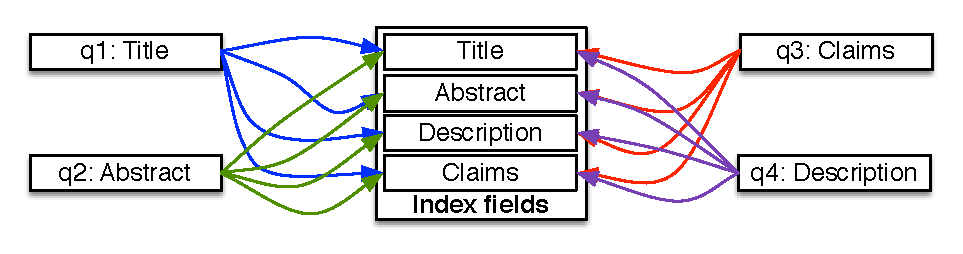
\includegraphics[width=8cm]{img/matching}%\par\end{centering}%\caption{Model of the index fields matching with queries .}%\label{fig:IndexFields}%\end{figure}


\subsection{Baselines}

We also want to compare the performance of the above patent specific
query reformulation methods described in Section~\ref{sec:QueryReformulation}
to general query reformulation methods. The selected baselines are
described below.


\subsubsection{Rocchio for Query Expansion}

The Rocchio algorithm \cite{Salton1971} is a classic algorithm of
relevance feedback used mainly for query expansion. Basically, it
provides a way of incorporating relevance feedback information into
the vector space model representing a query \cite{Manning2008}. We
refer to this method as \textbf{Rocchio}%
\footnote{We used the LucQE module, which provides an implementation of the
Rocchio method for Lucene. \\ \texttt{http://lucene-qe.sourceforge.net/}%
}.


\subsubsection{Rocchio for Query Reduction}

As a general QR method, we proposed to adapt the Rocchio method for
query pruning. Basically, the idea is once we have computed the Rocchio
modified query vector, we take only terms of the initial query that
appear in this vector and rank them using the Rocchio score. Then,
we remove $n$ terms with the lower score. We refer to this approach
as \textbf{RocchioQR}.


\subsection{Query Expansion Results}

In this section, we discuss the results of the evaluation performed
on the QE methods described above. But before, we first discuss the
effect of the size of the PRF set on the performance. Table \ref{tbl:PFRSize}
shows the impact of the PRF size on the performance for the two QE
algorithms Rocchio and MMRQE. These results are shown on the CLEF-IP
2010 training dataset, which consists of 196 topics. We observe that
the best QE performance results are obtained when using few documents
in the PRF set as it was also reported in \cite{Magdy2011} (in our
case, the top five gave the best results). This is certainly due to
the fact that a large PRF set will include too much irrelevant documents,
whose the terms may negatively affect the quality of the expanded
query.

\begin{table}[h]
\protect\caption{Effect of PRF with various numbers of feedback documents on the CLEF-IP
2010 dataset. 20 terms are used for query expansion.}
\label{tbl:PFRSize}

\centering{}{\scriptsize{}}%
\begin{tabular}{|l|c|c|c|c|c|}
\hline 
\textbf{\scriptsize{}Query/Source} & \textbf{\scriptsize{}Metric} & \textbf{\scriptsize{}Method} & \textbf{\scriptsize{}5} & \textbf{\scriptsize{}10} & \textbf{\scriptsize{}20}\tabularnewline
\hline 
\hline 
{\scriptsize{}Query: Abstract} & {\scriptsize{}MAP} & {\scriptsize{}Rocchio} & {\scriptsize{}0.074} & {\scriptsize{}0.072} & {\scriptsize{}0.070}\tabularnewline
\cline{3-6} 
 & {\scriptsize{}BL=0.073} & {\scriptsize{}MMRQE} & {\scriptsize{}0.074} & {\scriptsize{}0.071} & {\scriptsize{}0.071}\tabularnewline
\cline{2-6} 
{\scriptsize{}Source: Claims} & {\scriptsize{}PRES} & {\scriptsize{}Rocchio} & {\scriptsize{}0.409} & {\scriptsize{}0.409} & {\scriptsize{}0.409}\tabularnewline
\cline{3-6} 
 & \multirow{1}{*}{{\scriptsize{}BL=0.403}} & {\scriptsize{}MMRQE} & {\scriptsize{}0.411} & {\scriptsize{}0.411} & {\scriptsize{}0.410}\tabularnewline
\hline 
{\scriptsize{}Query: Claims} & {\scriptsize{}MAP} & {\scriptsize{}Rocchio} & {\scriptsize{}0.083} & {\scriptsize{}0.080} & {\scriptsize{}0.079}\tabularnewline
\cline{3-6} 
 & {\scriptsize{}BL=0.081} & {\scriptsize{}MMRQE} & {\scriptsize{}0.082} & {\scriptsize{}0.080} & {\scriptsize{}0.080}\tabularnewline
\cline{2-6} 
{\scriptsize{}Source: Claims} & {\scriptsize{}PRES} & {\scriptsize{}Rocchio} & {\scriptsize{}0.443} & {\scriptsize{}0.445} & {\scriptsize{}0.446}\tabularnewline
\cline{3-6} 
 & {\scriptsize{}BL=0.433} & {\scriptsize{}MMRQE} & {\scriptsize{}0.445} & {\scriptsize{}0.444} & {\scriptsize{}0.442}\tabularnewline
\hline 
\end{tabular}
\end{table}


\begin{comment}
As recommended in \cite{Magdy2012} and confirmed in our own experimentation
(not shown due to lack of space), best QE performance results are
obtained when using few documents in the PRF set (in our case, the
top five gave the best results).
\end{comment}
{} 

Next, we carry out comprehensive experiments with the following specific
options: 
\begin{itemize}
\item \textbf{Query type:} \{Title, Abstract, Claims, Description\}
\item \textbf{Query expansion source:} \{Abstract, Claims, Description\}
(considering that there is no interest in using the title as source
for the expansion)
\item \textbf{Relevance model:} \{BM25, Vector Space Model (VSM)\} 
\item \textbf{Term selection method:} \{Rocchio, MMRQE, IPC Codes, WSynSet,
USynSet\}
\end{itemize}
Figure \ref{fig:QE-qClaims-sAbstract-CLEF-2010} shows the results
obtained in terms of MAP and PRES for CLEF-IP 2010 for different numbers
of expanded terms $k$ on the x-axis (with $k=0$ using no QE, just
the baseline retrieval model). For lack of space we show only the
results of queries extracted from the claims and the abstract used
as source of query expansion. From these results, we make the following
observations: (i) for the two retrieval models (VSM and BM25), MMRQE
provides the best performance for both MAP and PRES (except for MAP,
where Rocchio BM25 provides better performance than MMRQE BM25), (ii)
for both MMRQE and Rocchio, the best performance is obtained while
adding no more than 50 terms to the original queries (adding more
terms may have no effect, or decrease the performance), and (iii)
exploiting external sources for query expansion provides poor performance
(IPC code definition and SynSets).

\begin{center}
\begin{figure}[h]
\begin{centering}
\includegraphics[width=4.3cm]{../CIKM2014/Results-CIKM2014/qClaims-sAbstract_MAP_2010}\includegraphics[width=4.3cm]{../CIKM2014/Results-CIKM2014/qClaims-sAbstract_PRES_2010}
\par\end{centering}

\protect\caption{Results obtained while using the claims for querying and the abstract
as source of query expansion on the CLEF-IP 2010 dataset.}


\label{fig:QE-qClaims-sAbstract-CLEF-2010}
\end{figure}

\par\end{center}

To summarize all the results obtained over all the above configurations,
Figures~\ref{fig:MAP-CLEF2010}, and ~\ref{fig:PRES-CLEF2010},
show the performance obtained for all the QE methods, while selecting
the optimal number of terms used for the expansion (number of terms
that maximizes the performance for each method). From these results,
we first observe that the best section to use for querying is the
description section (see Figures \ref{fig:qDescription-MAP-CLEF-IP2010},
and \ref{fig:qDescription-PRES-CLEF-IP2010}). We attribute this to
the fact that the description section has more content along with
relevant terms that define the invention since a detailed summary
of the invention is described therein.

According to our experiments, the best source for query expansion
is the claims section. We attribute this to the fact that, the claims
contain not only relevant, but also, specific terminology, since the
scope of the invention is described therein. However, when querying
using the claims, other sources of query expansion provided better
performance. This may be because claims are very similar between them
and contained specific terms; consequently, the queries lack of diversity
and general terms or synonyms that are used to describe similar inventions.
It is interesting to notice that the description is not either a good
source for expansion, since its content is too broad, therefore, it
contains many irrelevant terms that hurt the performance.

As expected, we observed that query expansion is not useful for very
long queries (i.e. description), indicating that in advanced stages
of the patent application process, QE is not relevant. We also notice
that when dealing with more mid-long queries such as abstract or claims,
MMRQE is more effective than Rocchio, which suggest that diverse term
selection is not crucial for short queries. We also note that using
the IPC code definitions (as suggested by \cite{Mahdabi2013}) and
SynSet (method of \cite{Magdy2011}) as a source of expansion, gave
poor performance (see IPC Codes and SynSet bars along the Figures).
Finally, regarding the best term selection method, we conclude that
in general MMRQE provides better performance than Rocchio.

%\begin{figure*}[t]
%\begin{centering}
%\subfigure[{\tiny Query Claims \& source Title.}]{\includegraphics[width=4.3cm]{Results-SIGIR2014/qClaims-sTitle_MAP_2011}}\subfigure[{\tiny Query Claims \& source Abstract.}]{\includegraphics[width=4.3cm]{Results-SIGIR2014/qClaims-sAbstract_MAP_2011}}\subfigure[{\tiny Query Claims \& source Claims.}]{\includegraphics[width=4.3cm]{Results-SIGIR2014/qClaims-sClaims_MAP_2011}}\subfigure[{\tiny Query Claims \& source Descrip.}]{\includegraphics[width=4.3cm]{Results-SIGIR2014/qClaims-sDescription_MAP_2011}}
%\par\end{centering}
%\vspace{-3mm}
%\caption{Mean Average Precision (MAP) on CLEF-2011 (for MMRQE $\lambda=0.5$).}
%\label{fig:MAP-CLEF2011}
%\vspace{-3mm}
%\end{figure*}


%\begin{figure*}
%\begin{centering}
%\subfigure[{\tiny Query Claims \& source Title.}]{\includegraphics[width=4.3cm]{Results-SIGIR2014/qClaims-sTitle_PRES_2011}}\subfigure[{\tiny Query Claims \& source Abstract.}]{\includegraphics[width=4.3cm]{Results-SIGIR2014/qClaims-sAbstract_PRES_2011}}\subfigure[{\tiny Query Claims \& source Claims.}]{\includegraphics[width=4.3cm]{Results-SIGIR2014/qClaims-sClaims_PRES_2011}}\subfigure[{\tiny Query Claims \& source Descrip.}]{\includegraphics[width=4.3cm]{Results-SIGIR2014/qClaims-sDescription_PRES_2011}}
%\par\end{centering}
%\vspace{-3mm}
%\caption{Patent Retrieval Evaluation Score (PRES) on CLEF-2011 (for MMRQE $\lambda=0.5$).}
%\label{fig:PRES-CLEF2011}
%\vspace{-3mm}
%r\end{figure*}



\subsection{Query Reduction Results}

In this section, we discuss the results of the evaluation performed
on the QR methods described above. As recommended in \cite{Ganguly2011}
and confirmed in our own experimentation (not shown due to lack of
space), best QR performance results are also obtained when using few
documents in the PRF set (in our case, the top five gave the best
results).

In the following, we carry out experiments with the following specific
options: 
\begin{itemize}
\item \textbf{Query type:} \{Title, Abstract, Claims, Description\} (considering
that there is no interest in reducing a title query)
\item \textbf{Relevance model:} \{BM25, Vector Space Model (VSM)\}
\item \textbf{Term selection method:} \{RocchioQR, MMRQR, LMQR, IPC Codes\} 
\end{itemize}
Figure \ref{fig:QR-qDescription-CLEF-2010} shows the results obtained
in terms of MAP and PRES for CLEF-IP 2010 for different numbers of
removed terms $k$ on the x-axis (with $k=0$ using no QR, just the
baseline retrieval model). For lack of space we show only the results
of queries extracted from the description. These results tell us mainly
two things: (i) for the two retrieval models, MMRQR provides the best
performance for both MAP and PRES, and (ii) for almost all methods,
the best performance is obtained when removing about 30 terms from
the original queries (in the case where the description is used for
querying). Removing more terms will decrease significantly the performance.

\begin{center}
\begin{figure}[t]
\begin{centering}
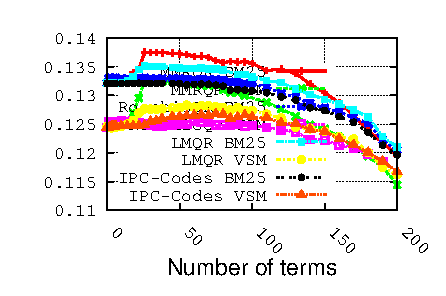
\includegraphics[width=4.3cm]{../CIKM2014/mmrqrResults/qDescription-sDescription_MAP_2010}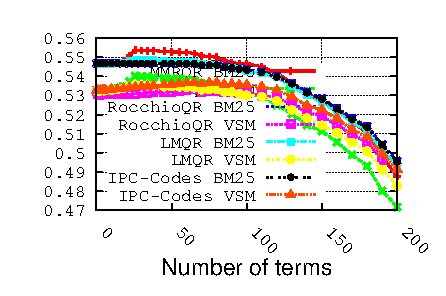
\includegraphics[width=4.3cm]{../CIKM2014/mmrqrResults/qDescription-sDescription_PRES_2010}
\par\end{centering}

\protect\caption{Results obtained for QR while using the description for querying on
the CLEF-IP 2010 dataset.}


\label{fig:QR-qDescription-CLEF-2010}
\end{figure}

\par\end{center}

To summarize all the results obtained over all the above configurations,
Figures \ref{fig:QR-PRES-CLEF-IP2010}, and \ref{fig:QR-MAP-CLEF-IP2010}
show the performance obtained for all the QR methods, when selecting
the optimal number of terms removed from the original queries (number
of terms removed that maximizes the performance for each method).

From these results, we make the following observations: (i) query
reduction is very often not useful for short queries (i.e. title),
since no QR method outperforms significantly the baseline (i.e. No
QR), (ii) when dealing with very long query (i.e. description), BM25
based QR methods perform better than VSM based QR methods, and (iii)
in general, MMRQR provides better performance than the other methods.


\section{Conclusion}

\label{sec:conclusion}

In this paper we analyzed general and specific query reformulation
methods for patent prior art search for partial (incomplete) patent
applications on two patent retrieval corpora, namely CLEF-IP 2010
and CLEF-IP 2011. We demonstrated that QE methods are critical for
short queries, i.e. title, abstract, and claims, but useless for very
long queries, i.e. the description section. We also showed that claims
is the best section that works with QE both to query with and to use
as a source of query expansion terms, suggesting that claims should
be written at early stages of the patent application drafting so that
they can be use to performed patent prior art search. In the same
vein, we also found that the patent specific fields are more suited
as a source for expansion than external sources such as synonym dictionaries.
Here, future work concerns how can we exploit patent specific meta-data
such as inventor and citation networks for query expansion

Regarding QR methods, we showed that these techniques are effective
to some extent for claims and description sections, which are considered
the longest sections in a patent application. Future work may consist
of exploiting query quality predictors to identify useless terms in
a query using machine learning methods.

{\scriptsize{} \bibliographystyle{abbrv}
\bibliography{biblio}
}{\scriptsize \par}

\begin{figure*}
\begin{centering}
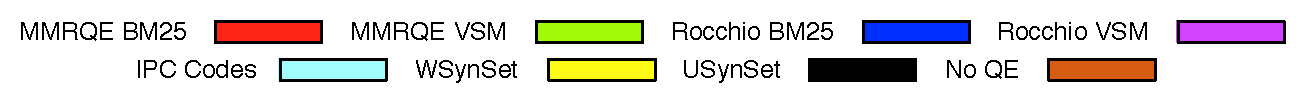
\includegraphics[width=12cm]{img/legendQE} 
\par\end{centering}

\begin{centering}
\subfloat[Query Title.]{\begin{centering}
\includegraphics[width=6cm]{Results-CIKM2014/qTitle-MAP-CLEF-IP2010} 
\par\end{centering}

}\subfloat[Query Abstract.]{\begin{centering}
\includegraphics[width=6cm]{Results-CIKM2014/qAbstract-MAP-CLEF-IP2010} 
\par\end{centering}

\label{fig:qDescription-MAP-CLEF-IP2010}}
\par\end{centering}

\begin{centering}
\subfloat[Query Claims.]{\begin{centering}
\includegraphics[width=6cm]{Results-CIKM2014/qClaims-MAP-CLEF-IP2010} 
\par\end{centering}

}\subfloat[Query Description.]{\begin{centering}
\includegraphics[width=6cm]{Results-CIKM2014/qDescription-MAP-CLEF-IP2010} 
\par\end{centering}

}
\par\end{centering}

\protect\caption{MAP for QE methods on CLEF-IP 2010.}


\label{fig:MAP-CLEF2010} 
\end{figure*}


\begin{figure*}
\begin{centering}
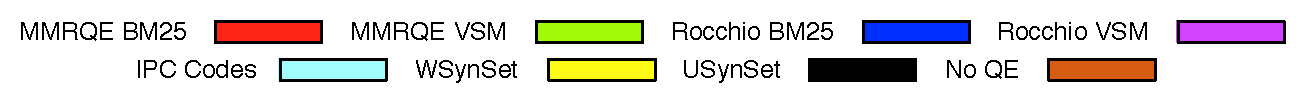
\includegraphics[width=12cm]{img/legendQE} 
\par\end{centering}

\begin{centering}
\subfloat[Query Title.]{\begin{centering}
\includegraphics[width=6cm]{Results-CIKM2014/qTitle-PRES-CLEF-IP2010} 
\par\end{centering}

}\subfloat[Query Abstract.]{\begin{centering}
\includegraphics[width=6cm]{Results-CIKM2014/qAbstract-PRES-CLEF-IP2010} 
\par\end{centering}

}
\par\end{centering}

\begin{centering}
\subfloat[Query Claims.]{\begin{centering}
\includegraphics[width=6cm]{Results-CIKM2014/qClaims-PRES-CLEF-IP2010} 
\par\end{centering}

}\subfloat[Query Description.]{\begin{centering}
\includegraphics[width=6cm]{Results-CIKM2014/qDescription-PRES-CLEF-IP2010} 
\par\end{centering}

\label{fig:qDescription-PRES-CLEF-IP2010}}
\par\end{centering}

\protect\caption{PRES for QE methods on CLEF-IP 2010.}


\label{fig:PRES-CLEF2010} 
\end{figure*}
\begin{comment}
\begin{figure*}
\begin{centering}
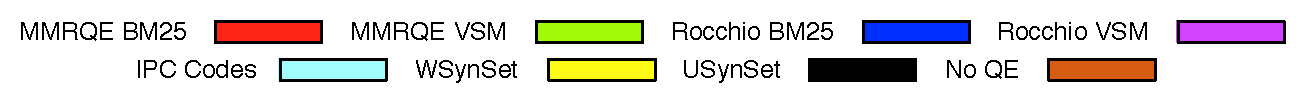
\includegraphics[width=12cm]{img/legendQE.eps} 
\par\end{centering}

\begin{centering}
\subfloat[Query Title.]{\begin{centering}
\includegraphics[width=6cm]{Results-CIKM2014/qTitle-MAP-CLEF-IP2011.eps} 
\par\end{centering}

}\subfloat[Query Abstract.]{\begin{centering}
\includegraphics[width=6cm]{Results-CIKM2014/qAbstract-MAP-CLEF-IP2011.eps} 
\par\end{centering}

}
\par\end{centering}

\begin{centering}
\subfloat[Query Claims.]{\begin{centering}
\includegraphics[width=6cm]{Results-CIKM2014/qClaims-MAP-CLEF-IP2011.eps} 
\par\end{centering}

}\subfloat[Query Description.]{\begin{centering}
\includegraphics[width=6cm]{Results-CIKM2014/qDescription-MAP-CLEF-IP2011.eps} 
\par\end{centering}

}
\par\end{centering}

\begin{centering}
\label{fig:qDescription-MAP-CLEF-IP2011} 
\par\end{centering}

\protect\caption{MAP for QE methods on CLEF-IP 2011.}


\label{fig:MAP-CLEF2011} 
\end{figure*}


\begin{figure*}
\begin{centering}
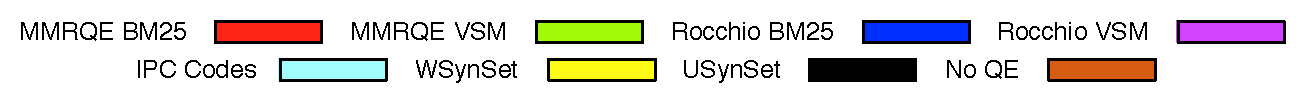
\includegraphics[width=12cm]{img/legendQE.eps} 
\par\end{centering}

\begin{centering}
\subfloat[Query Title.]{\begin{centering}
\includegraphics[width=6cm]{Results-CIKM2014/qTitle-PRES-CLEF-IP2011.eps} 
\par\end{centering}

}\subfloat[Query Abstract.]{\begin{centering}
\includegraphics[width=6cm]{Results-CIKM2014/qAbstract-PRES-CLEF-IP2011.eps} 
\par\end{centering}

}
\par\end{centering}

\begin{centering}
\subfloat[Query Claims.]{\begin{centering}
\includegraphics[width=6cm]{Results-CIKM2014/qClaims-PRES-CLEF-IP2011.eps} 
\par\end{centering}

}\subfloat[Query Description.]{\begin{centering}
\includegraphics[width=6cm]{Results-CIKM2014/qDescription-PRES-CLEF-IP2011.eps} 
\par\end{centering}

}
\par\end{centering}

\begin{centering}
\label{fig:qDescription-PRES-CLEF-IP2011} 
\par\end{centering}

\protect\caption{PRES for QE methods on CLEF 2011.}


\label{fig:PRES-CLEF2011} 
\end{figure*}
\end{comment}


\begin{figure*}
\begin{centering}
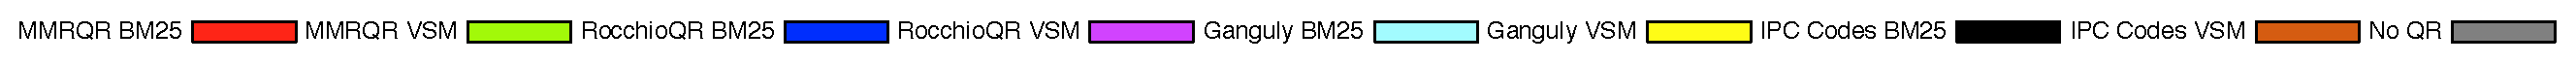
\includegraphics[width=12cm]{img/legendQR} 
\par\end{centering}

\begin{centering}
\subfloat[Query Abstract.]{\begin{centering}
\includegraphics[width=4cm]{mmrqrResults/qAbstract-MAP-CLEF-IP2010} 
\par\end{centering}

}\subfloat[Query Claims.]{\begin{centering}
\includegraphics[width=4cm]{mmrqrResults/qClaims-MAP-CLEF-IP2010} 
\par\end{centering}

}\subfloat[Query Description.]{\begin{centering}
\includegraphics[width=4cm]{mmrqrResults/qDescription-MAP-CLEF-IP2010} 
\par\end{centering}

}
\par\end{centering}

\protect\caption{MAP for QR methods on CLEF-IP 2010.}


\label{fig:QR-PRES-CLEF-IP2010} 
\end{figure*}


\begin{figure*}
\begin{centering}
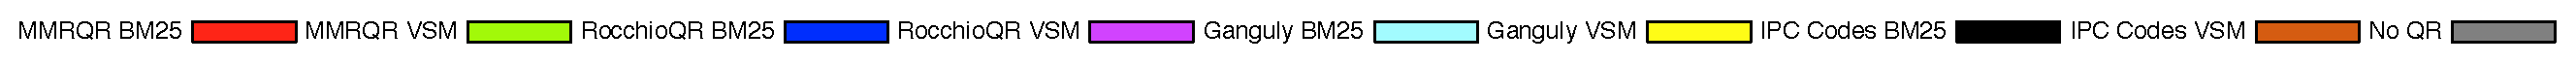
\includegraphics[width=12cm]{img/legendQR} 
\par\end{centering}

\begin{centering}
\subfloat[Query Abstract.]{\begin{centering}
\includegraphics[width=4cm]{mmrqrResults/qAbstract-PRES-CLEF-IP2010} 
\par\end{centering}

}\subfloat[Query Claims.]{\begin{centering}
\includegraphics[width=4cm]{mmrqrResults/qClaims-PRES-CLEF-IP2010} 
\par\end{centering}

}\subfloat[Query Description.]{\begin{centering}
\includegraphics[width=4cm]{mmrqrResults/qDescription-PRES-CLEF-IP2010} 
\par\end{centering}

}
\par\end{centering}

\protect\caption{PRES for QR methods on CLEF 2010.}


\label{fig:QR-MAP-CLEF-IP2010} 
\end{figure*}
\begin{comment}
\begin{figure*}
\begin{centering}
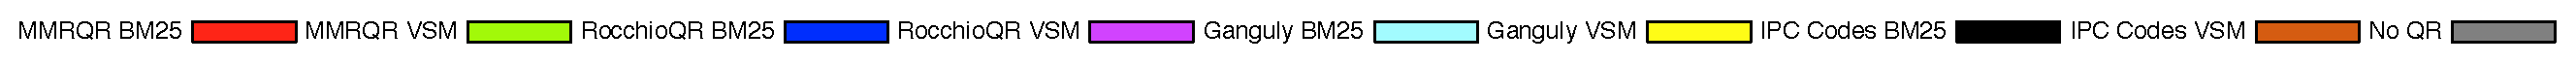
\includegraphics[width=12cm]{img/legendQR.eps} 
\par\end{centering}

\begin{centering}
\subfloat[Query Abstract.]{\begin{centering}
\includegraphics[width=4cm]{mmrqrResults/qAbstract-MAP-CLEF-IP2011.eps} 
\par\end{centering}

}\subfloat[Query Claims.]{\begin{centering}
\includegraphics[width=4cm]{mmrqrResults/qClaims-MAP-CLEF-IP2011.eps} 
\par\end{centering}

}\subfloat[Query Description.]{\begin{centering}
\includegraphics[width=4cm]{mmrqrResults/qDescription-MAP-CLEF-IP2011.eps} 
\par\end{centering}

}
\par\end{centering}

\protect\caption{MAP for QR methods on CLEF-IP 2011.}


\label{fig:QR-PRES-CLEF-IP2011} 
\end{figure*}


\begin{figure*}
\begin{centering}
\includegraphics[width=12cm]{img/legendQR.eps} 
\par\end{centering}

\begin{centering}
\subfloat[Query Abstract.]{\begin{centering}
\includegraphics[width=4cm]{mmrqrResults/qAbstract-PRES-CLEF-IP2011.eps} 
\par\end{centering}

}\subfloat[Query Claims.]{\begin{centering}
\includegraphics[width=4cm]{mmrqrResults/qClaims-PRES-CLEF-IP2011.eps} 
\par\end{centering}

}\subfloat[Query Description.]{\begin{centering}
\includegraphics[width=4cm]{mmrqrResults/qDescription-PRES-CLEF-IP2011.eps} 
\par\end{centering}

}
\par\end{centering}

\protect\caption{PRES for QR methods on CLEF 2011.}


\label{fig:QR-MAP-CLEF-IP2011} 
\end{figure*}
\end{comment}


\clearpage{}

\begin{comment}
\begin{figure*}[t]
\begin{centering}
\subfigure[{\tiny Query Title \& source Title.}]{\includegraphics[width=4.3cm,bb = 0 0 200 100, draft, type=eps]{../Results-CIKM2014/qTitle-sTitle_MAP_2010.eps}}\subfigure[{\tiny Query Title \& source Abstract.}]{\includegraphics[width=4.3cm,bb = 0 0 200 100, draft, type=eps]{../Results-CIKM2014/qTitle-sAbstract_MAP_2010.eps}}\subfigure[{\tiny Query Title \& source Claims.}]{\includegraphics[width=4.3cm,bb = 0 0 200 100, draft, type=eps]{../Results-CIKM2014/qTitle-sClaims_MAP_2010.eps}}\subfigure[{\tiny Query Title \& source Descrip.}]{\includegraphics[width=4.3cm,bb = 0 0 200 100, draft, type=eps]{../Results-CIKM2014/qTitle-sDescription_MAP_2010.eps}} 
\par\end{centering}

\begin{centering}
\subfigure[{\tiny Query Abstract \& source Title.}]{\includegraphics[width=4.3cm,bb = 0 0 200 100, draft, type=eps]{../Results-CIKM2014/qAbstract-sTitle_MAP_2010.eps}}\subfigure[{\tiny Query Abstract \& source Abstract.}]{\includegraphics[width=4.3cm,bb = 0 0 200 100, draft, type=eps]{../Results-CIKM2014/qAbstract-sAbstract_MAP_2010.eps}}\subfigure[{\tiny Query Abstract \& source Claims.}]{\includegraphics[width=4.3cm,bb = 0 0 200 100, draft, type=eps]{../Results-CIKM2014/qAbstract-sClaims_MAP_2010.eps}}\subfigure[{\tiny Query Abstract \& source Descrip.}]{\includegraphics[width=4.3cm,bb = 0 0 200 100, draft, type=eps]{../Results-CIKM2014/qAbstract-sDescription_MAP_2010.eps}} 
\par\end{centering}

\begin{centering}
\subfigure[{\tiny Query Claims \& source Title.}]{\includegraphics[width=4.3cm,bb = 0 0 200 100, draft, type=eps]{../Results-CIKM2014/qClaims-sTitle_MAP_2010.eps}}\subfigure[{\tiny Query Claims \& source Abstract.}]{\includegraphics[width=4.3cm,bb = 0 0 200 100, draft, type=eps]{../Results-CIKM2014/qClaims-sAbstract_MAP_2010.eps}}\subfigure[{\tiny Query Claims \& source Claims.}]{\includegraphics[width=4.3cm,bb = 0 0 200 100, draft, type=eps]{../Results-CIKM2014/qClaims-sClaims_MAP_2010.eps}}\subfigure[{\tiny Query Claims \& source Descrip.}]{\includegraphics[width=4.3cm,bb = 0 0 200 100, draft, type=eps]{../Results-CIKM2014/qClaims-sDescription_MAP_2010.eps}}
\subfigure[{\tiny Query Descrip \& source Title.}]{\includegraphics[width=4.3cm,bb = 0 0 200 100, draft, type=eps]{../Results-CIKM2014/qDescription-sTitle_MAP_2010.eps}}\subfigure[{\tiny Query Descrip \& source Abstract.}]{\includegraphics[width=4.3cm,bb = 0 0 200 100, draft, type=eps]{../Results-CIKM2014/qDescription-sAbstract_MAP_2010.eps}}\subfigure[{\tiny Query Descrip \& source Claims.}]{\includegraphics[width=4.3cm,bb = 0 0 200 100, draft, type=eps]{../Results-CIKM2014/qDescription-sClaims_MAP_2010.eps}}\subfigure[{\tiny Query Descrip \& source Descrip.}]{\includegraphics[width=4.3cm,bb = 0 0 200 100, draft, type=eps]{../Results-CIKM2014/qDescription-sDescription_MAP_2010.eps}} 
\par\end{centering}

\protect\caption{Mean Average Precision (MAP) on CLEF-2010 (for MMRQE $\lambda=0.5$).}


\label{fig:MAP-CLEF2010-1} 
\end{figure*}


\begin{figure*}
\begin{centering}
\subfigure[{\tiny Query Title \& source Title.}]{\includegraphics[width=4.3cm,bb = 0 0 200 100, draft, type=eps]{../Results-CIKM2014/qTitle-sTitle_PRES_2010.eps}}\subfigure[{\tiny Query Title \& source Abstract.}]{\includegraphics[width=4.3cm,bb = 0 0 200 100, draft, type=eps]{../Results-CIKM2014/qTitle-sAbstract_PRES_2010.eps}}\subfigure[{\tiny Query Title \& source Claims.}]{\includegraphics[width=4.3cm,bb = 0 0 200 100, draft, type=eps]{../Results-CIKM2014/qTitle-sClaims_PRES_2010.eps}}\subfigure[{\tiny Query Title \& source Descrip.}]{\includegraphics[width=4.3cm,bb = 0 0 200 100, draft, type=eps]{../Results-CIKM2014/qTitle-sDescription_PRES_2010.eps}} 
\par\end{centering}

\begin{centering}
\subfigure[{\tiny Query Abstract \& source Title.}]{\includegraphics[width=4.3cm,bb = 0 0 200 100, draft, type=eps]{../Results-CIKM2014/qAbstract-sTitle_PRES_2010.eps}}\subfigure[{\tiny Query Abstract \& source Abstract.}]{\includegraphics[width=4.3cm,bb = 0 0 200 100, draft, type=eps]{../Results-CIKM2014/qAbstract-sAbstract_PRES_2010.eps}}\subfigure[{\tiny Query Abstract \& source Claims.}]{\includegraphics[width=4.3cm,bb = 0 0 200 100, draft, type=eps]{../Results-CIKM2014/qAbstract-sClaims_PRES_2010.eps}}\subfigure[{\tiny Query Abstract \& source Descrip.}]{\includegraphics[width=4.3cm,bb = 0 0 200 100, draft, type=eps]{../Results-CIKM2014/qAbstract-sDescription_PRES_2010.eps}} 
\par\end{centering}

\begin{centering}
\subfigure[{\tiny Query Claims \& source Title.}]{\includegraphics[width=4.3cm,bb = 0 0 200 100, draft, type=eps]{../Results-CIKM2014/qClaims-sTitle_PRES_2010.eps}}\subfigure[{\tiny Query Claims \& source Abstract.}]{\includegraphics[width=4.3cm,bb = 0 0 200 100, draft, type=eps]{../Results-CIKM2014/qClaims-sAbstract_PRES_2010.eps}}\subfigure[{\tiny Query Claims \& source Claims.}]{\includegraphics[width=4.3cm,bb = 0 0 200 100, draft, type=eps]{../Results-CIKM2014/qClaims-sClaims_PRES_2010.eps}}\subfigure[{\tiny Query Claims \& source Descrip.}]{\includegraphics[width=4.3cm,bb = 0 0 200 100, draft, type=eps]{../Results-CIKM2014/qClaims-sDescription_PRES_2010.eps}}
\subfigure[{\tiny Query Descrip \& source Title.}]{\includegraphics[width=4.3cm,bb = 0 0 200 100, draft, type=eps]{../Results-CIKM2014/qDescription-sTitle_PRES_2010.eps}}\subfigure[{\tiny Query Descrip \& source Abstract.}]{\includegraphics[width=4.3cm,bb = 0 0 200 100, draft, type=eps]{../Results-CIKM2014/qDescription-sAbstract_PRES_2010.eps}}\subfigure[{\tiny Query Descrip \& source Claims.}]{\includegraphics[width=4.3cm,bb = 0 0 200 100, draft, type=eps]{../Results-CIKM2014/qDescription-sClaims_PRES_2010.eps}}\subfigure[{\tiny Query Descrip \& source Descrip.}]{\includegraphics[width=4.3cm,bb = 0 0 200 100, draft, type=eps]{../Results-CIKM2014/qDescription-sDescription_PRES_2010.eps}} 
\par\end{centering}

\protect\caption{Patent Retrieval Evaluation Score (PRES) on CLEF-2010 (for MMRQE $\lambda=0.5$).}


\label{fig:PRES-CLEF2010-1} 
\end{figure*}


\begin{figure*}[t]
\begin{centering}
\subfigure[{\tiny Query Title \& source Title.}]{\includegraphics[width=4.3cm,bb = 0 0 200 100, draft, type=eps]{../Results-CIKM2014/qTitle-sTitle_MAP_2011.eps}}\subfigure[{\tiny Query Title \& source Abstract.}]{\includegraphics[width=4.3cm,bb = 0 0 200 100, draft, type=eps]{../Results-CIKM2014/qTitle-sAbstract_MAP_2011.eps}}\subfigure[{\tiny Query Title \& source Claims.}]{\includegraphics[width=4.3cm,bb = 0 0 200 100, draft, type=eps]{../Results-CIKM2014/qTitle-sClaims_MAP_2011.eps}}\subfigure[{\tiny Query Title \& source Descrip.}]{\includegraphics[width=4.3cm,bb = 0 0 200 100, draft, type=eps]{../Results-CIKM2014/qTitle-sDescription_MAP_2011.eps}} 
\par\end{centering}

\begin{centering}
\subfigure[{\tiny Query Abstract \& source Title.}]{\includegraphics[width=4.3cm,bb = 0 0 200 100, draft, type=eps]{../Results-CIKM2014/qAbstract-sTitle_MAP_2011.eps}}\subfigure[{\tiny Query Abstract \& source Abstract.}]{\includegraphics[width=4.3cm,bb = 0 0 200 100, draft, type=eps]{../Results-CIKM2014/qAbstract-sAbstract_MAP_2011.eps}}\subfigure[{\tiny Query Abstract \& source Claims.}]{\includegraphics[width=4.3cm,bb = 0 0 200 100, draft, type=eps]{../Results-CIKM2014/qAbstract-sClaims_MAP_2011.eps}}\subfigure[{\tiny Query Abstract \& source Descrip.}]{\includegraphics[width=4.3cm,bb = 0 0 200 100, draft, type=eps]{../Results-CIKM2014/qAbstract-sDescription_MAP_2011.eps}} 
\par\end{centering}

\begin{centering}
\subfigure[{\tiny Query Claims \& source Title.}]{\includegraphics[width=4.3cm,bb = 0 0 200 100, draft, type=eps]{../Results-CIKM2014/qClaims-sTitle_MAP_2011.eps}}\subfigure[{\tiny Query Claims \& source Abstract.}]{\includegraphics[width=4.3cm,bb = 0 0 200 100, draft, type=eps]{../Results-CIKM2014/qClaims-sAbstract_MAP_2011.eps}}\subfigure[{\tiny Query Claims \& source Claims.}]{\includegraphics[width=4.3cm,bb = 0 0 200 100, draft, type=eps]{../Results-CIKM2014/qClaims-sClaims_MAP_2011.eps}}\subfigure[{\tiny Query Claims \& source Descrip.}]{\includegraphics[width=4.3cm,bb = 0 0 200 100, draft, type=eps]{../Results-CIKM2014/qClaims-sDescription_MAP_2011.eps}}
\subfigure[{\tiny Query Descrip \& source Title.}]{\includegraphics[width=4.3cm,bb = 0 0 200 100, draft, type=eps]{../Results-CIKM2014/qDescription-sTitle_MAP_2011.eps}}\subfigure[{\tiny Query Descrip \& source Abstract.}]{\includegraphics[width=4.3cm,bb = 0 0 200 100, draft, type=eps]{../Results-CIKM2014/qDescription-sAbstract_MAP_2011.eps}}\subfigure[{\tiny Query Descrip \& source Claims.}]{\includegraphics[width=4.3cm,bb = 0 0 200 100, draft, type=eps]{../Results-CIKM2014/qDescription-sClaims_MAP_2011.eps}}\subfigure[{\tiny Query Descrip \& source Descrip.}]{\includegraphics[width=4.3cm,bb = 0 0 200 100, draft, type=eps]{../Results-CIKM2014/qDescription-sDescription_MAP_2011.eps}} 
\par\end{centering}

\protect\caption{Mean Average Precision (MAP) on CLEF-2011 (for MMRQE $\lambda=0.5$).}
\end{figure*}


\begin{figure*}
\begin{centering}
\subfigure[{\tiny Query Title \& source Title.}]{\includegraphics[width=4.3cm,bb = 0 0 200 100, draft, type=eps]{../Results-CIKM2014/qTitle-sTitle_PRES_2011.eps}}\subfigure[{\tiny Query Title \& source Abstract.}]{\includegraphics[width=4.3cm,bb = 0 0 200 100, draft, type=eps]{../Results-CIKM2014/qTitle-sAbstract_PRES_2011.eps}}\subfigure[{\tiny Query Title \& source Claims.}]{\includegraphics[width=4.3cm,bb = 0 0 200 100, draft, type=eps]{../Results-CIKM2014/qTitle-sClaims_PRES_2011.eps}}\subfigure[{\tiny Query Title \& source Descrip.}]{\includegraphics[width=4.3cm,bb = 0 0 200 100, draft, type=eps]{../Results-CIKM2014/qTitle-sDescription_PRES_2011.eps}} 
\par\end{centering}

\begin{centering}
\subfigure[{\tiny Query Abstract \& source Title.}]{\includegraphics[width=4.3cm,bb = 0 0 200 100, draft, type=eps]{../Results-CIKM2014/qAbstract-sTitle_PRES_2011.eps}}\subfigure[{\tiny Query Abstract \& source Abstract.}]{\includegraphics[width=4.3cm,bb = 0 0 200 100, draft, type=eps]{../Results-CIKM2014/qAbstract-sAbstract_PRES_2011.eps}}\subfigure[{\tiny Query Abstract \& source Claims.}]{\includegraphics[width=4.3cm,bb = 0 0 200 100, draft, type=eps]{../Results-CIKM2014/qAbstract-sClaims_PRES_2011.eps}}\subfigure[{\tiny Query Abstract \& source Descrip.}]{\includegraphics[width=4.3cm,bb = 0 0 200 100, draft, type=eps]{../Results-CIKM2014/qAbstract-sDescription_PRES_2011.eps}} 
\par\end{centering}

\begin{centering}
\subfigure[{\tiny Query Claims \& source Title.}]{\includegraphics[width=4.3cm,bb = 0 0 200 100, draft, type=eps]{../Results-CIKM2014/qClaims-sTitle_PRES_2011.eps}}\subfigure[{\tiny Query Claims \& source Abstract.}]{\includegraphics[width=4.3cm,bb = 0 0 200 100, draft, type=eps]{../Results-CIKM2014/qClaims-sAbstract_PRES_2011.eps}}\subfigure[{\tiny Query Claims \& source Claims.}]{\includegraphics[width=4.3cm,bb = 0 0 200 100, draft, type=eps]{../Results-CIKM2014/qClaims-sClaims_PRES_2011.eps}}\subfigure[{\tiny Query Claims \& source Descrip.}]{\includegraphics[width=4.3cm,bb = 0 0 200 100, draft, type=eps]{../Results-CIKM2014/qClaims-sDescription_PRES_2011.eps}}
\subfigure[{\tiny Query Descrip \& source Title.}]{\includegraphics[width=4.3cm,bb = 0 0 200 100, draft, type=eps]{../Results-CIKM2014/qDescription-sTitle_PRES_2011.eps}}\subfigure[{\tiny Query Descrip \& source Abstract.}]{\includegraphics[width=4.3cm,bb = 0 0 200 100, draft, type=eps]{../Results-CIKM2014/qDescription-sAbstract_PRES_2011.eps}}\subfigure[{\tiny Query Descrip \& source Claims.}]{\includegraphics[width=4.3cm,bb = 0 0 200 100, draft, type=eps]{../Results-CIKM2014/qDescription-sClaims_PRES_2011.eps}}\subfigure[{\tiny Query Descrip \& source Descrip.}]{\includegraphics[width=4.3cm,bb = 0 0 200 100, draft, type=eps]{../Results-CIKM2014/qDescription-sDescription_PRES_2011.eps}} 
\par\end{centering}

\protect\caption{Patent Retrieval Evaluation Score (PRES) on CLEF-2011 (for MMRQE $\lambda=0.5$).}
\end{figure*}
\end{comment}


\clearpage{}

\begin{comment}
\begin{figure*}[t]
\begin{centering}
\subfigure[{Query Title.}]{\includegraphics[width=4.3cm,bb = 0 0 200 100, draft, type=eps]{../mmrqrResults/qTitle-sDescription_MAP_2010.eps}}\subfigure[{Query Abstract.}]{\includegraphics[width=4.3cm,bb = 0 0 200 100, draft, type=eps]{../mmrqrResults/qAbstract-sDescription_MAP_2010.eps}}\subfigure[{Query Claims.}]{\includegraphics[width=4.3cm,bb = 0 0 200 100, draft, type=eps]{../mmrqrResults/qClaims-sDescription_MAP_2010.eps}}
\subfigure[{Query Description.}]{\includegraphics[width=4.3cm,bb = 0 0 200 100, draft, type=eps]{../mmrqrResults/qDescription-sDescription_MAP_2010.eps}} 
\par\end{centering}

\protect\caption{Mean Average Precision (MAP) for MMRQR on CLEF-2010 (for MMRQE $\lambda=0.8$).}
\end{figure*}


\begin{figure*}
\begin{centering}
\subfigure[{ Query Title.}]{\includegraphics[width=4.3cm,bb = 0 0 200 100, draft, type=eps]{../mmrqrResults/qTitle-sDescription_PRES_2010.eps}}\subfigure[{Query Abstract.}]{\includegraphics[width=4.3cm,bb = 0 0 200 100, draft, type=eps]{../mmrqrResults/qAbstract-sDescription_PRES_2010.eps}}\subfigure[{Query Claims.}]{\includegraphics[width=4.3cm,bb = 0 0 200 100, draft, type=eps]{../mmrqrResults/qClaims-sDescription_PRES_2010.eps}}
\subfigure[{Query Description.}]{\includegraphics[width=4.3cm,bb = 0 0 200 100, draft, type=eps]{../mmrqrResults/qDescription-sDescription_PRES_2010.eps}} 
\par\end{centering}

\protect\caption{Patent Retrieval Evaluation Score (PRES) for MMRQR on CLEF-2010 (for
MMRQE $\lambda=0.8$).}
\end{figure*}


\begin{figure*}[t]
\begin{centering}
\subfigure[{Query Title.}]{\includegraphics[width=4.3cm,bb = 0 0 200 100, draft, type=eps]{../mmrqrResults/qTitle-sDescription_MAP_2011.eps}}\subfigure[{Query Abstract.}]{\includegraphics[width=4.3cm,bb = 0 0 200 100, draft, type=eps]{../mmrqrResults/qAbstract-sDescription_MAP_2011.eps}}\subfigure[{Query Claims.}]{\includegraphics[width=4.3cm,bb = 0 0 200 100, draft, type=eps]{../mmrqrResults/qClaims-sDescription_MAP_2011.eps}}
\subfigure[{Query Description.}]{\includegraphics[width=4.3cm,bb = 0 0 200 100, draft, type=eps]{../mmrqrResults/qDescription-sDescription_MAP_2011.eps}} 
\par\end{centering}

\protect\caption{Mean Average Precision (MAP) for MMRQR on CLEF-2011 (for MMRQE $\lambda=0.8$).}
\end{figure*}


\begin{figure*}
\begin{centering}
\subfigure[{ Query Title.}]{\includegraphics[width=4.3cm,bb = 0 0 200 100, draft, type=eps]{../mmrqrResults/qTitle-sDescription_PRES_2011.eps}}\subfigure[{Query Abstract.}]{\includegraphics[width=4.3cm,bb = 0 0 200 100, draft, type=eps]{../mmrqrResults/qAbstract-sDescription_PRES_2011.eps}}\subfigure[{Query Claims.}]{\includegraphics[width=4.3cm,bb = 0 0 200 100, draft, type=eps]{../mmrqrResults/qClaims-sDescription_PRES_2011.eps}}
\subfigure[{Query Description.}]{\includegraphics[width=4.3cm,bb = 0 0 200 100, draft, type=eps]{../mmrqrResults/qDescription-sDescription_PRES_2011.eps}} 
\par\end{centering}

\protect\caption{Patent Retrieval Evaluation Score (PRES) for MMRQR on CLEF-2011 (for
MMRQE $\lambda=0.8$).}
\end{figure*}
\end{comment}

\end{document}
